\documentclass{beamer}
\usepackage{beamerthemesplit} % new 
\usepackage{graphicx}
\usepackage{caption}
%\usepackage{subcaption}
\usepackage{lmodern}
\usepackage{color}
\usetheme{Pittsburgh}
\usecolortheme{dolphin}

% citations
\usepackage[]{natbib}


\title[HFT Experiments: Testing FBA]{Experiments in High-Frequency Trading: \\ Testing the Frequent Batch Auction}
\author[Aldrich, L\'opez Vargas]{Eric M. Aldrich\inst{1} \and Kristian L\'opez Vargas\inst{1}}
\institute[UCSC]{\inst{1} Economics Department, University of California, Santa Cruz  }
\useoutertheme{infolines}


\begin{document}

\date{BEEC - January 2019} 

\frame{\titlepage} 


\section{Summary}
\frame{\frametitle{One-slide Summary}
\begin{itemize}
\item \textbf{HFT}: "trading that uses powerful computers to transact a large number of orders at fractions of a second." (Now more than 50\% of traded volume worldwide)
% \pause

\item \textbf{Broad Motivation:} What is a good design for financial markets in the presence of HFT? Does the CDA/CLOB exhibit important flaws? What are the alternative market formats? 

% \pause
\item \textbf{This paper:} A laboratory study that compares the CDA against a (newly) proposed Frequent Batch Auction (FBA). 

% \pause
\item \textbf{Results:} The FBA outperforms the CDA. FBA exhibits:

\begin{enumerate}
\item less \textbf{predatory} trading behavior
\item less wasteful investments in \textbf{communication} technology.
\item lower \textbf{transacting costs} (spread)
\item lower \textbf{volatility}, higher market \textbf{stability}
\end{enumerate}
\end{itemize}
}

\section{Introduction} 



% \frame{\frametitle{The HFT Debate} 
% \begin{itemize}
% \item Exchanges (NYSE et al.) automated order execution about 20 years ago, substantially reducing spreads and latencies. 
% \item Today, most trades involve low latency, automated traders: the HFT industry.
% \item HFT firms provide liquidity, although not cheaply, and this liquidity may be illusory. Overall, actual transactions costs are not necessarily lowest under the current market design and with HFTs.
% \item HFT firms \textit{might} be destabilizing the markets (as in the 2010 ``flash crash'').
% \item Regulators seem to take these fears seriously, and are considering heavy handed ``fixes''.
% \end{itemize}
% }

\frame{\frametitle{Motivation: A piece of the HFT Debate} 

\begin{itemize}
\item The CDA/CLOB has a \textbf{design flaw} (Budish et al. 2015). 
% \pause
\item Huge \textbf{Rewards}  for traders that can react to information a nanosecond \textbf{faster} than others and exploit stale orders. 
% \pause
\item This generates an \textbf{arms race} around expensive faster communication technology.
% \pause
\item The outcome: a \textbf{massive prisoner's dilemma}
% \pause
\item Are there other market rules that undo the negative incentives built-in the CDA? Yes: \textbf{FBA}, IEX, Flow markets, etc.

\item Existing data cannot resolve the debate, as data come from a single exchange format. 

\item Experimentation allows us to generate evidence on the relative performance of market alternatives.	

\end{itemize}
}

%In March 2014, New York City Attorney General Eric Schneiderman launched a probe of HFT-related practices; so far he has served subpoenas on the largest HFT firms, exchanges and banks operating dark pools and 
% filed a lawsuit against Barclays, alleging that the bank illicitly operated its dark pool in ways to favor HFT. 
% In June 2016, the U.S. Securities and Exchange Commission approved a plan put forth by IEX, a new trading venue, to delay all incoming orders with the intention of reducing the advantage of HFT firms. 
%In July 2016, India?s regulators announced plans to create similar ?speed bumps? for their major financial markets. Regulators around the world are contemplating similar moves.

\section{Experiment Design}

% \frame{\frametitle{Environment: Basics} 
% Orders:
% \begin{enumerate}
% \item limit order: example: "BUY, up to \$101, 20 Units, GTC"
% \item market order: example: "BUY, up to $\infty$, 30 Units, IOC"
% \end{enumerate}
% \vspace{5mm}
% Latencies: \\
% Time elapsed between sending and receiving the order, and between receipt and processing.
% }


\subsection{Environment}


\frame{\frametitle{Experiment Environment: BCS 
- Exogenous Processes} 
Budish, Cramton and Shim (QJE, 2015, hereafter BCS) \\
There is one \textbf{single asset}, trades in a single exchange. \\
Two exogenous processes generate incentives to trade:
\begin{enumerate}

\item the fundamental value of the asset, $V(t)$
\begin{itemize}
\item publicly observed
\item evolves over continuous time following a compound Poisson jump process
\item arrival rate of $\lambda_V$ per second and jump distribution $F_{V}$
\end{itemize} 


\item a population of investors (noise traders) that
\begin{itemize}
\item arrive at random times with Poisson rate of $\lambda_{I}$ per second, 
\item each places a unit market order to buy or sell with equal probability.
\end{itemize} 

\end{enumerate}
Profits are generated from reversing positions with respect to the fundamental value.
% Human participants play the role of trading firms and, at any instant, can choose whether
% \begin{itemize}
% \item to exit the market (out)
% \item to participate as a market maker
% \item or as a sniper
% \end{itemize}

}


\frame{\frametitle{Experiment Environment BCS: Exogenous Processes} 
\begin{itemize}
\item V(t) (jump rate $\lambda_V$, Jump ~ $N(0,\sigma^2)$)
\item Investor arrivals (arrival rate $\lambda_I$)
\end{itemize}

\begin{figure}
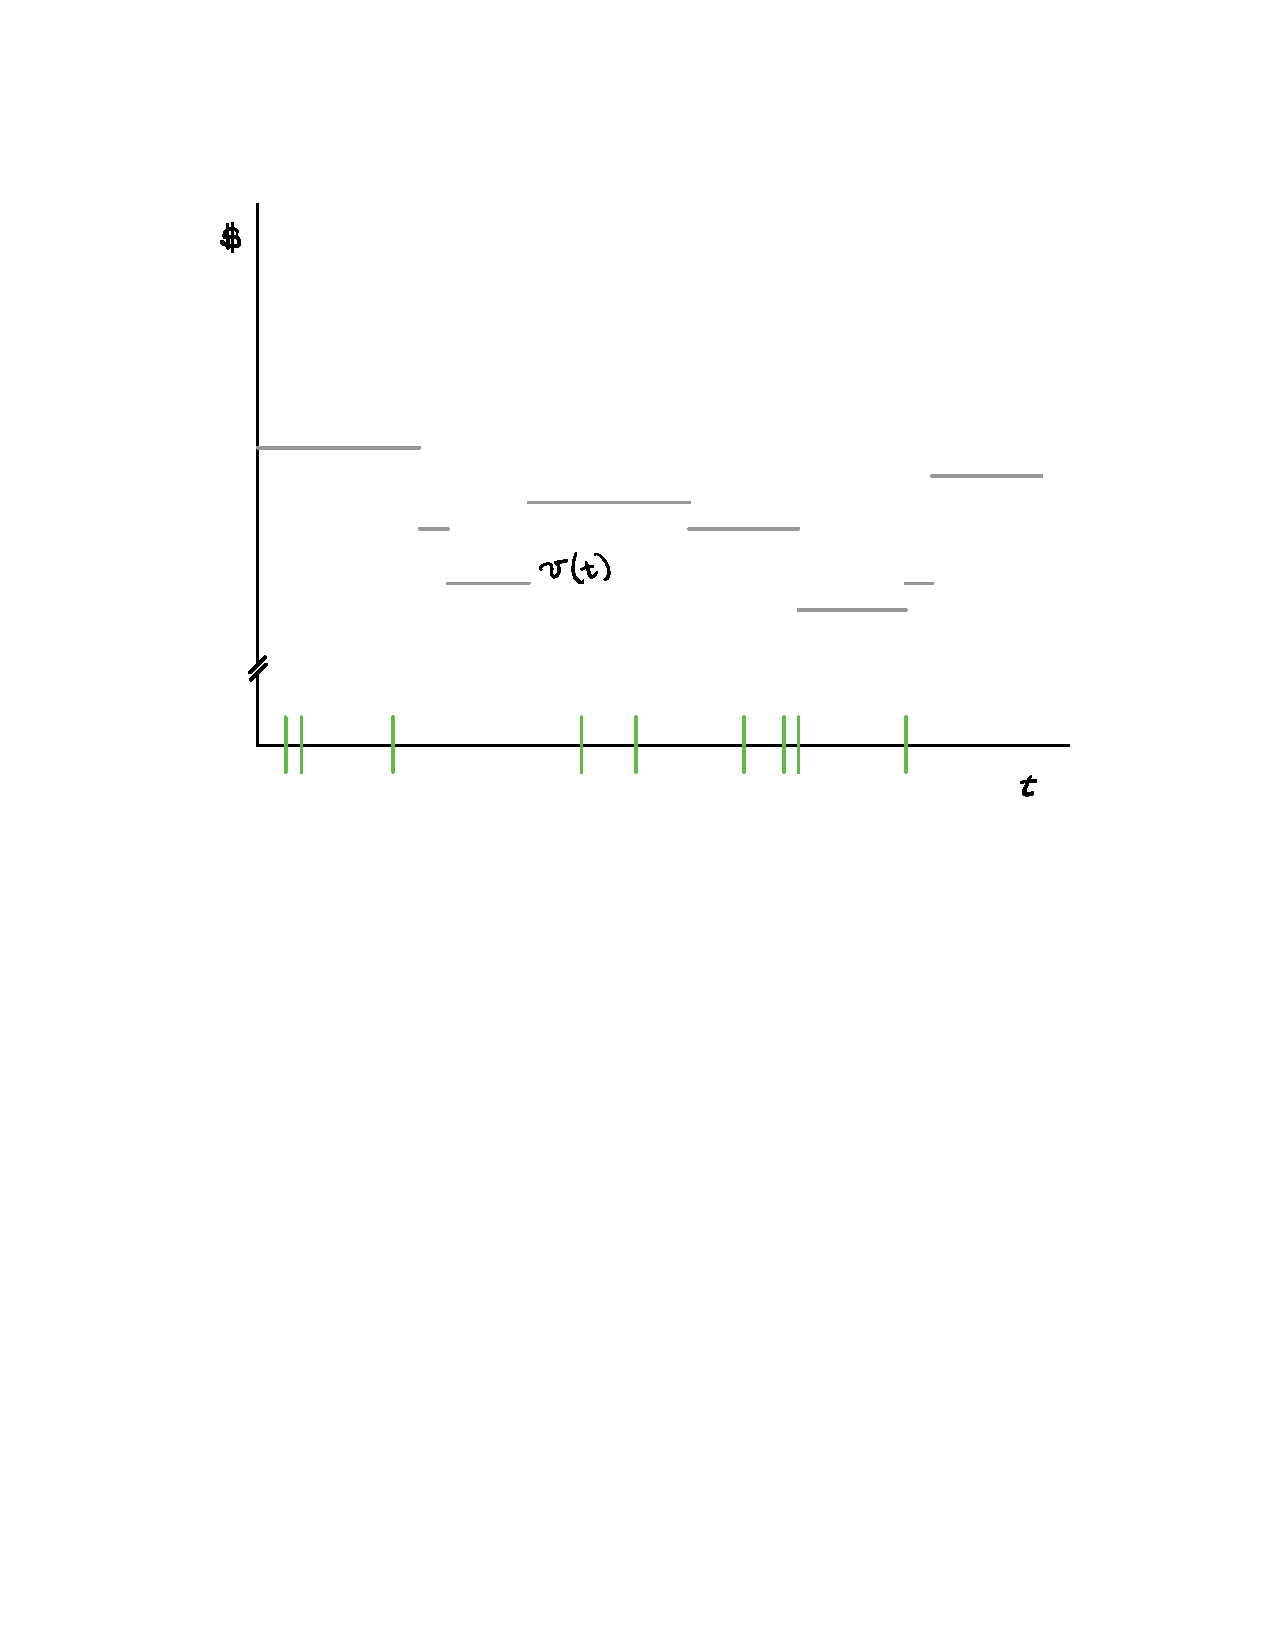
\includegraphics[width=0.7\textwidth]{img/two_processes.pdf}
\end{figure}
} 


\frame{\frametitle{Experiment Environment BCS: orders}
Limit orders, market orders and latencies (slow and fast).
\begin{figure}
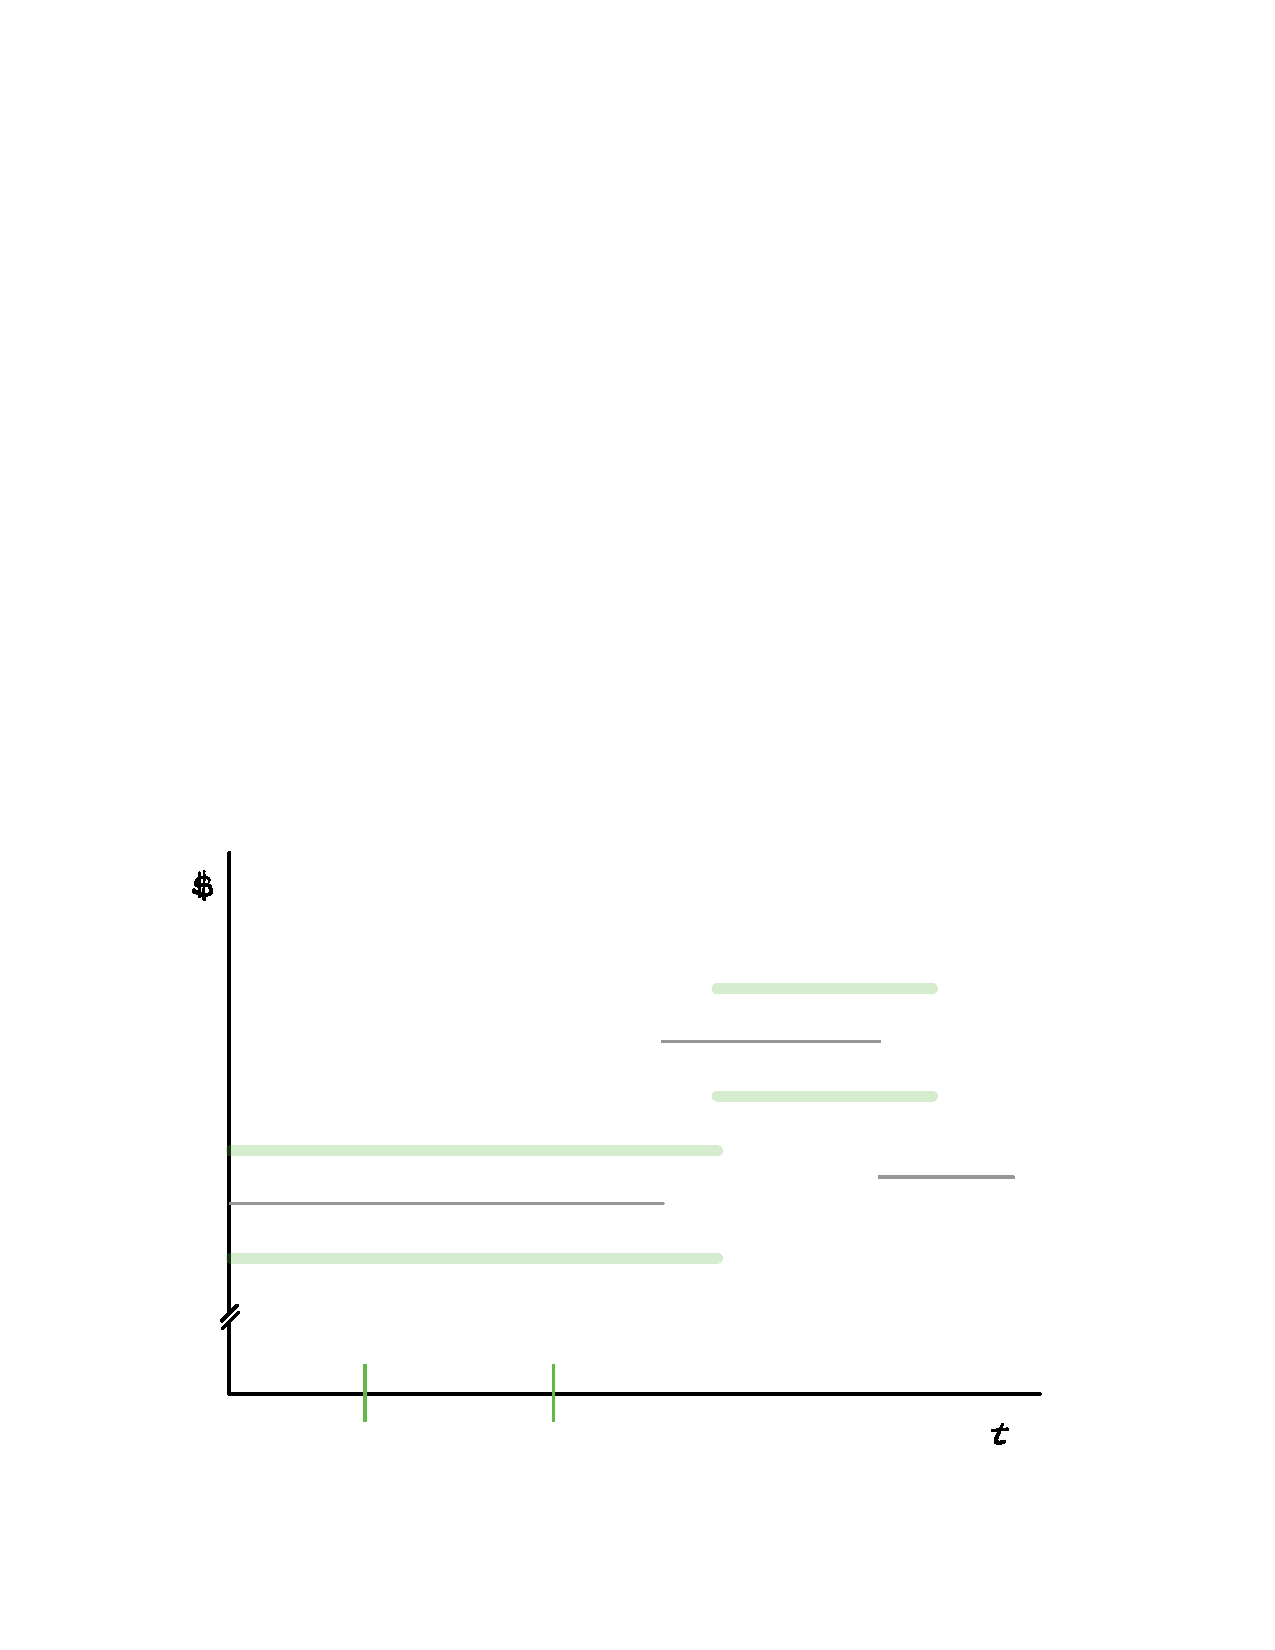
\includegraphics[width=0.7\textwidth]{img/buy_sell.pdf}
\end{figure}
}


\subsection{Auction Formats: CDA}

\frame{\frametitle{Market Format 1: The CDA} 
Continuous Double Auction (CDA): 
\begin{itemize}
\item Trade can happen at any moment of time. 
\item Strict price, time priority. 
% \item Market makers: post buy/sell limit orders that remain in the book. 
% \item Takers: submit market orders to transact immediately. 
\end{itemize} 
Trading strategies: 
\begin{itemize}
\item exit the market (out)
\item market maker
\item sniper
\end{itemize}
Technology strategy:
\begin{itemize}
\item Traders can subscribe to faster (lower-latency) communication technology at a cost of $c_{speed}$ per second.
\end{itemize}
\centering 
\textbf{There is value to reacting faster to public signal} \\

}



\frame{\frametitle{Market Format 1: The CDA} 
Investor arrivals and value jumps in the CDA.
\hyperlink{CDA_Equil}{\beamergotobutton{Equilibrium}}
\begin{figure}
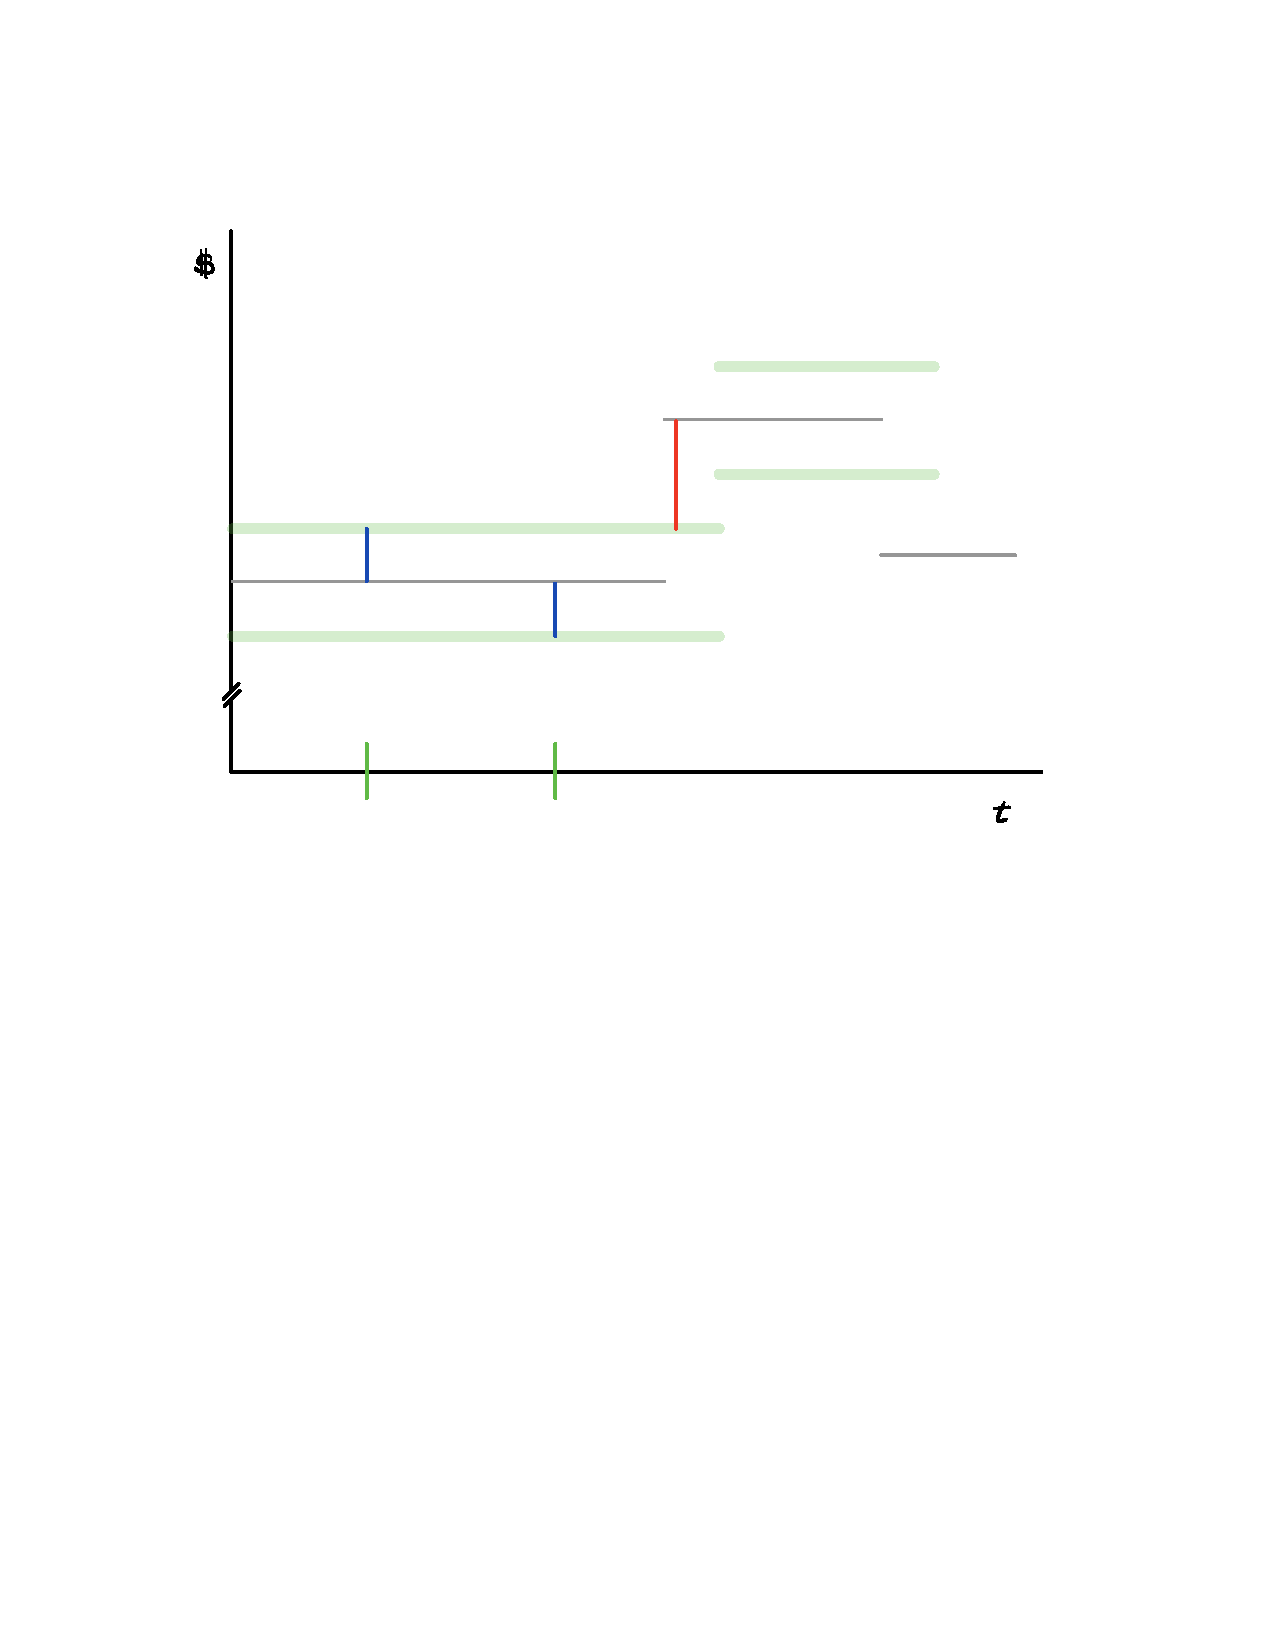
\includegraphics[width=0.7\textwidth]{img/CDA_diagram_events.pdf}
\end{figure}
}



% \frame{\frametitle{Market Format 1: The CDA} 
% Investor events:
% \begin{itemize}
% \item Investors' sell orders transact with the highest maker bid and buy orders transact with the lowest maker offer. 
% \item The maker with smallest spread, $s$, books profit $0.5s$ at a rate dictated by $\lambda_{I}$. 
% \end{itemize}
% Value jumps:
% \begin{itemize}
% \item At the moment of a sufficiently large positive (negative) change in the fundamental value($|\Delta V(t)| = |V(t)-V(t^{-})| > 0.5s$) snipers attempt to trade with the lowest ask (or highest bid) in the book.
% \item If this attempt is executed, we say a maker has been "sniped". Losses/gains = $|\Delta V(t)|-0.5s$ 
% \end{itemize}
% Ties are resolved randomly. \\
% }

\frame[label={CDA_Equil}]{\frametitle{Market Format 1: The CDA} 

Equilibrium in BCS environment under CDA:
\begin{itemize}
\item Finite numbers of participants $N^*$
\item All $N$ traders purchase fast communication technology
\item Only one trader plays market maker 
\item $N-1$ are snipers.
\item Free entry. Every trader earns zero profits. 
\item The cost of speed, purchased by all traders, is borne entirely by investors via market spread.
\item $s^*>0$, $\lambda_I \frac{s^*}{2} = N^* c_s$ 

\end{itemize}

}

% \frame{\frametitle{Market Format 1: The CDA} 

% Equilibrium is characterized by two zero-profit conditions. \\
% For the maker,
% \begin{equation}
%   \lambda_{I} \cdot \frac{s}{2} - 
%   \lambda_V    \cdot    \textrm{Pr}\left(J > \frac{s}{2}\right)    \cdot    E \left[J-\frac{s}{2} | J>\frac{s}{2}\right] 
%   \cdot    \frac{N-1}{N}   =   c_s, 
%   \label{eq:CDAmakerProfit}
% \end{equation}
% I.e.: expected profits from trading with investors minus the expected losses to snipers equal to the cost of buying speed services.
% }

% \frame{\frametitle{Market Format 1: The CDA} 
% For the sniper,
% \begin{align}
% \lambda_V \cdot \textrm{Pr}\left(J > \frac{s}{2}\right) \cdot E\left[J-\frac{s}{2}|J>\frac{s}{2}\right] \cdot \frac{1}{N} & = c_s, \label{eq:CDAsniperProfit}
% \end{align}
% I.e.: profits from sniping must be equal to expenditure on speed services. \\
% \vspace{5mm}
% Notice that all traders are subject to identical communication latency $\delta_{fast}$, causing the messages of all $N$ players to arrive in the exchange at the same time.
% }

% \frame{\frametitle{Market Format 1: The CDA} 
% Equilibrium in BCS environment under CDA: \\
% \begin{itemize}
% \item $N*$ traders in the market. One market maker, $N*-1$ snipers. \\ 
% \item Every trader invests in speed technology. \\
% \end{itemize}

% Rearrangement of equations \eqref{eq:CDAmakerProfit} and \eqref{eq:CDAsniperProfit} gives: 
% \begin{align}
% \lambda_I \cdot \frac{s^*}{2} & = 
% \lambda_V \cdot \textrm{Pr}\left(J > \frac{s^*}{2}\right) \cdot E\left[J-\frac{s^*}{2}|J>\frac{s^*}{2}\right] \label{eq:BCS1} \\
% \lambda_I \cdot \frac{s^*}{2} & = N^* c_s. \label{eq:BCS2}
% \end{align}

% Equation \eqref{eq:BCS1} determines $s^*$ and Equation \eqref{eq:BCS2} determines $N^*$. \\
% \vspace{5mm}

% Intuition: The cost of speed, purchased by all traders, is borne entirely by investors via market spread. 
% }

%%%%%%%%%%%%%%%%%%%%%%%%%%%%%%%%%%%%%%%%%%%%%%%%%%%%

\subsection{Auction Formats: FBA}

\frame[label={FBA}]{\frametitle{Market Format 2: The FBA} 
Frequent Batch Auction (FBA): 
\begin{itemize}
\item Trading day is divided in \textbf{many uniform price double auctions}:
\item Trade does NOT happen at any moment of time, but \textbf{periodically} (say, each tenth of a second), with a batching period for each auction.
\item At the end of the batching period, supply and demand cross and \textbf{market clears}. 
\end{itemize}
\begin{figure}
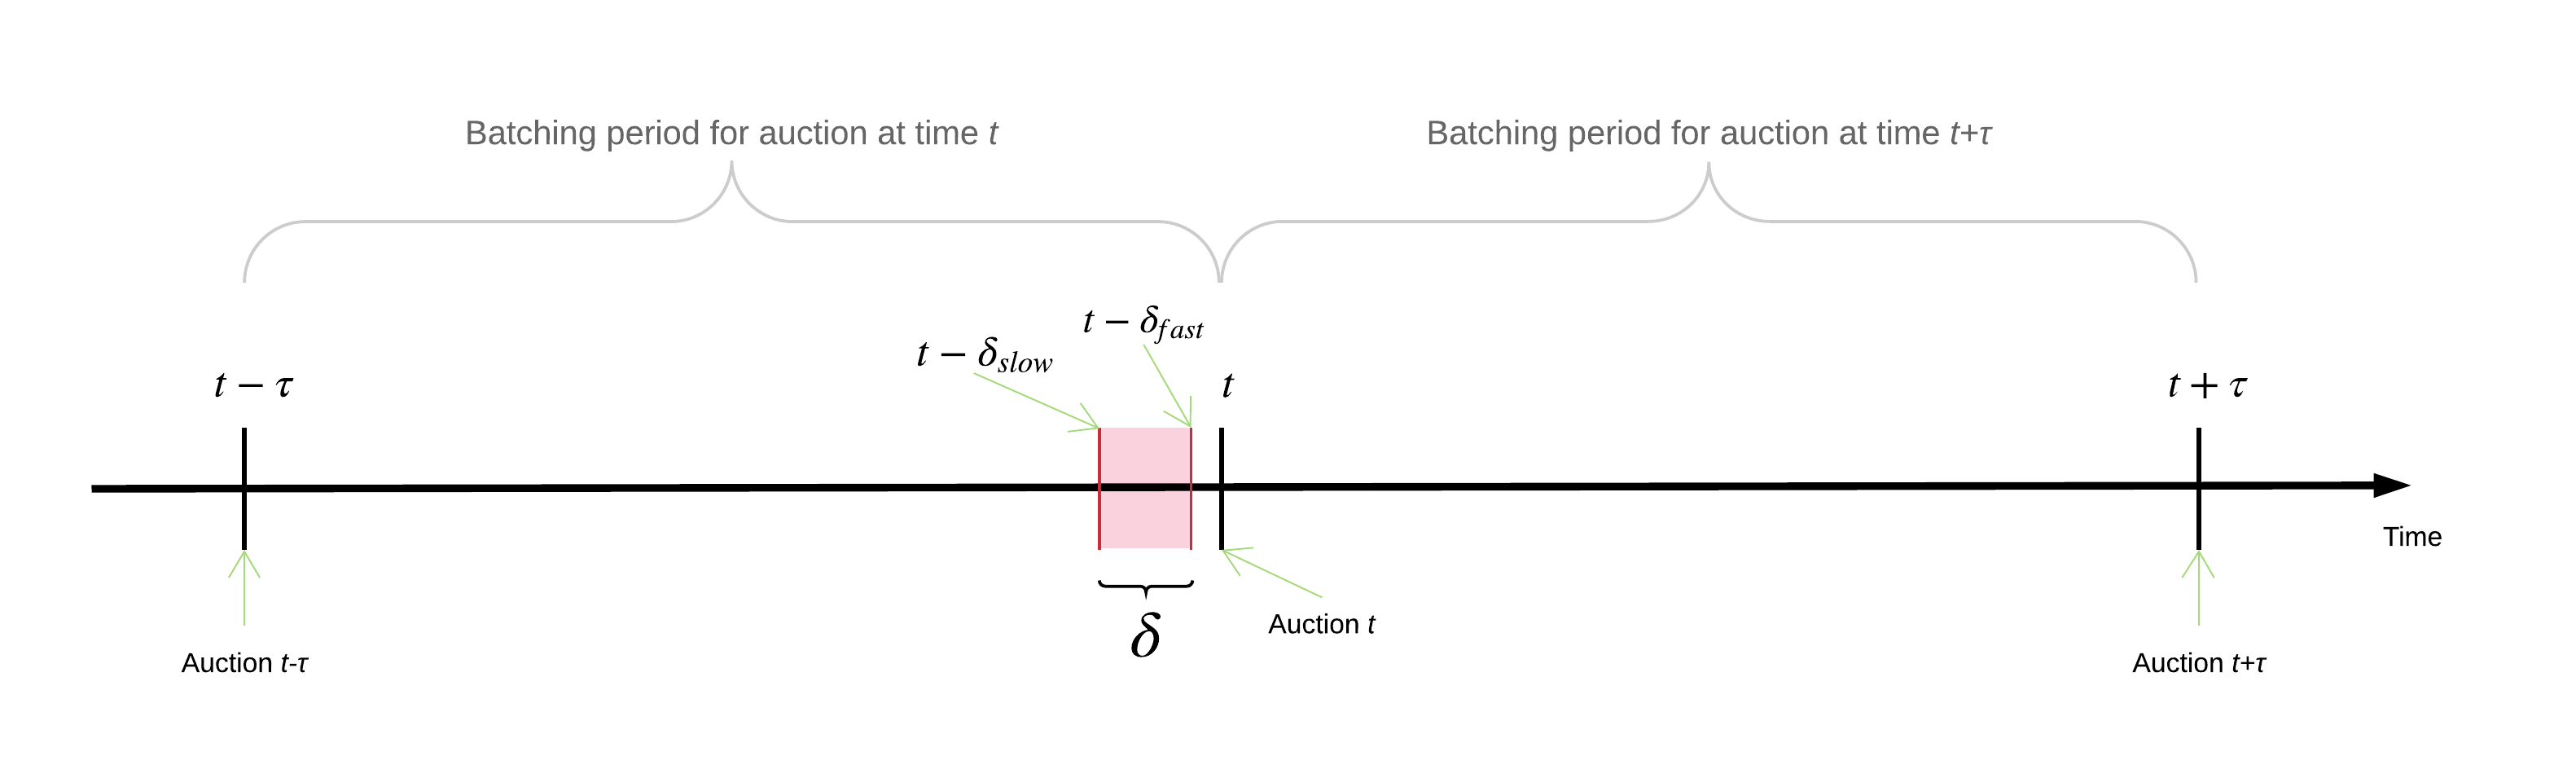
\includegraphics[width=0.8\textwidth]{img/timing_FBA.png}
\caption{\label{fig:FBAtiming}Timing in the FBA format (adapted from Budish et al. (2015)).}
\label{fig:fbaDiagram}
\end{figure}
}


\frame{\frametitle{Market Format 2: The FBA} 
Investor arrivals and value jumps in the FBA
\begin{figure}
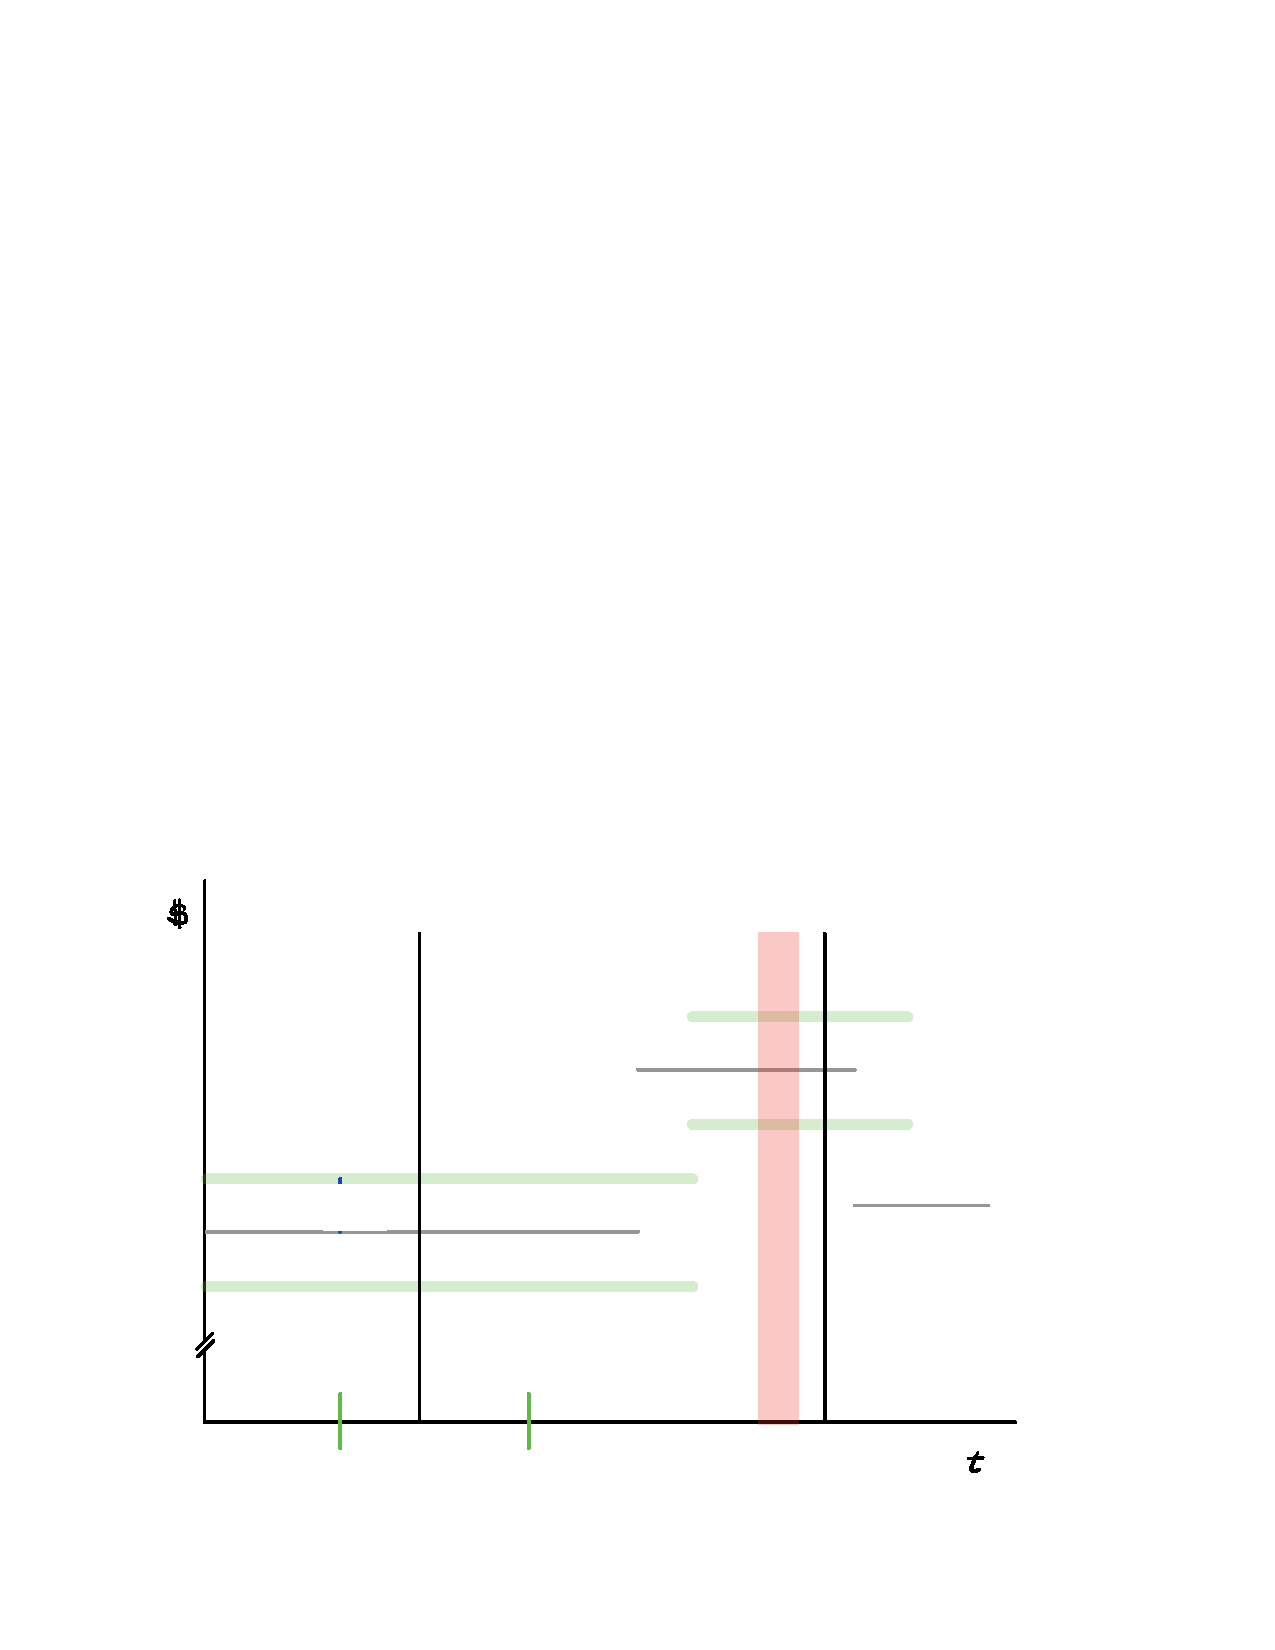
\includegraphics[width=0.7\textwidth]{img/FBA_diagram_events.pdf}
\end{figure}
}

\frame{\frametitle{Market Format 2: The FBA} 

Strategy space is the same as in the CDA \\

\vspace{5mm}

Equilibrium of the FBA in the BCS environment: \\
\begin{itemize}
\item Everyone is a \textit{slow maker} with zero spread ($s^*=0$). 
\item There are no sniper
\item No one purchases fast technology.
\item True if the batching period is substantially larger than default communication latency. \newline
\end{itemize}

}

% \frame{\frametitle{Market Format 2: The FBA} 

% Technically, the condition is (Budish et al., 2015) :
% \begin{align} 
% \label{eq:BCSFBA}
% \frac{\delta}{\tau} \cdot \lambda_V E\left[J | J>0\right] < c_s
% \end{align}
% I.e., there is no incentive for traders to take the role of a fast sniper in the FBA.
% }


\section{Experiment Design} 



%%%%%%%%%%%%%%%%%%%

\frame{\frametitle{Experiment } 
Choice Space: \\
Human subjects choose between 3 roles:
\begin{enumerate}
\item Out: stay out of the market
\item Maker: Post buy/sell orders at $V \pm s/2$, can freely update $s$.\\ 
With lag $\delta$, bot updates when $V$ jumps.\\ 
\item Sniper: Try to pick off stale quotes when $V$ jumps.
\end{enumerate}  

\vspace{8mm}
Speed subscription: 
\begin{itemize}
\item at flow cost $c>0$, reduce latency $\delta_{slow}$ to $\delta_{fast}$. \\
\end{itemize}
}

\frame{\frametitle{Treatments, Sessions}
\begin{itemize}
\item Six treatments $\{CDA,FBA\} \times \{C1,C2,C3\}$.
\item Between-subjects design
\item Group size = 6; fixed-group matching.
\item A session = eight consecutive trading periods of four minutes each 
\item Data for 24 markets or groups (4 groups per treatment, 12 sessions total).
\item Initial endowment: 20 ECUs; Exchange rate: 2 ECUs = 1 USD; 
\item Subjects paid for one randomly chosen period plus 7 USD. 
\item  Summary information between periods.
\item Sessions conducted at the LEEPS Laboratory at UCSC.
\end{itemize}
}

\frame{\frametitle{Treatments, Sessions}
\begin{table}[]
\centering
\begin{tabular}{lccc}
\hline
                                        & Config 1              & Config 2              & Config 3              \\ \hline
Parameters:                             &                       &                       &                       \\ 
%\multicolumn{1}{|c|}{
$ \ \ \ \ \ \lambda_{I}$ & 1/3                   & 1/5                   & 1/2                   \\ 
%\multicolumn{1}{|c|}{$ \\ \lambda_{V}$} 
$ \ \ \ \ \ \lambda_{V}$ & 1/4                   & 1                     & 1                     \\ 
%\multicolumn{1}{|c|}{$ \\ c_{speed}$} 
$ \ \ \ \ \  c_{speed}$   & 0.01                  & 0.01                & 0.022                 \\ 
Number of trading periods               & 8                     & 8                     & 8                     \\ 
Trading period length (secs)            & 240                   & 240                   & 240                   \\ 
                                        & 		 				& 	 					&  						\\ 
Groups (sessions) per treatment            & 4 (2)                 & 4 (2)                 & 4 (2)                 \\ \hline
\end{tabular}
\end{table}
}



\frame{\frametitle{CDA User Interface}
%\begin{itemize}\item 
%\centering
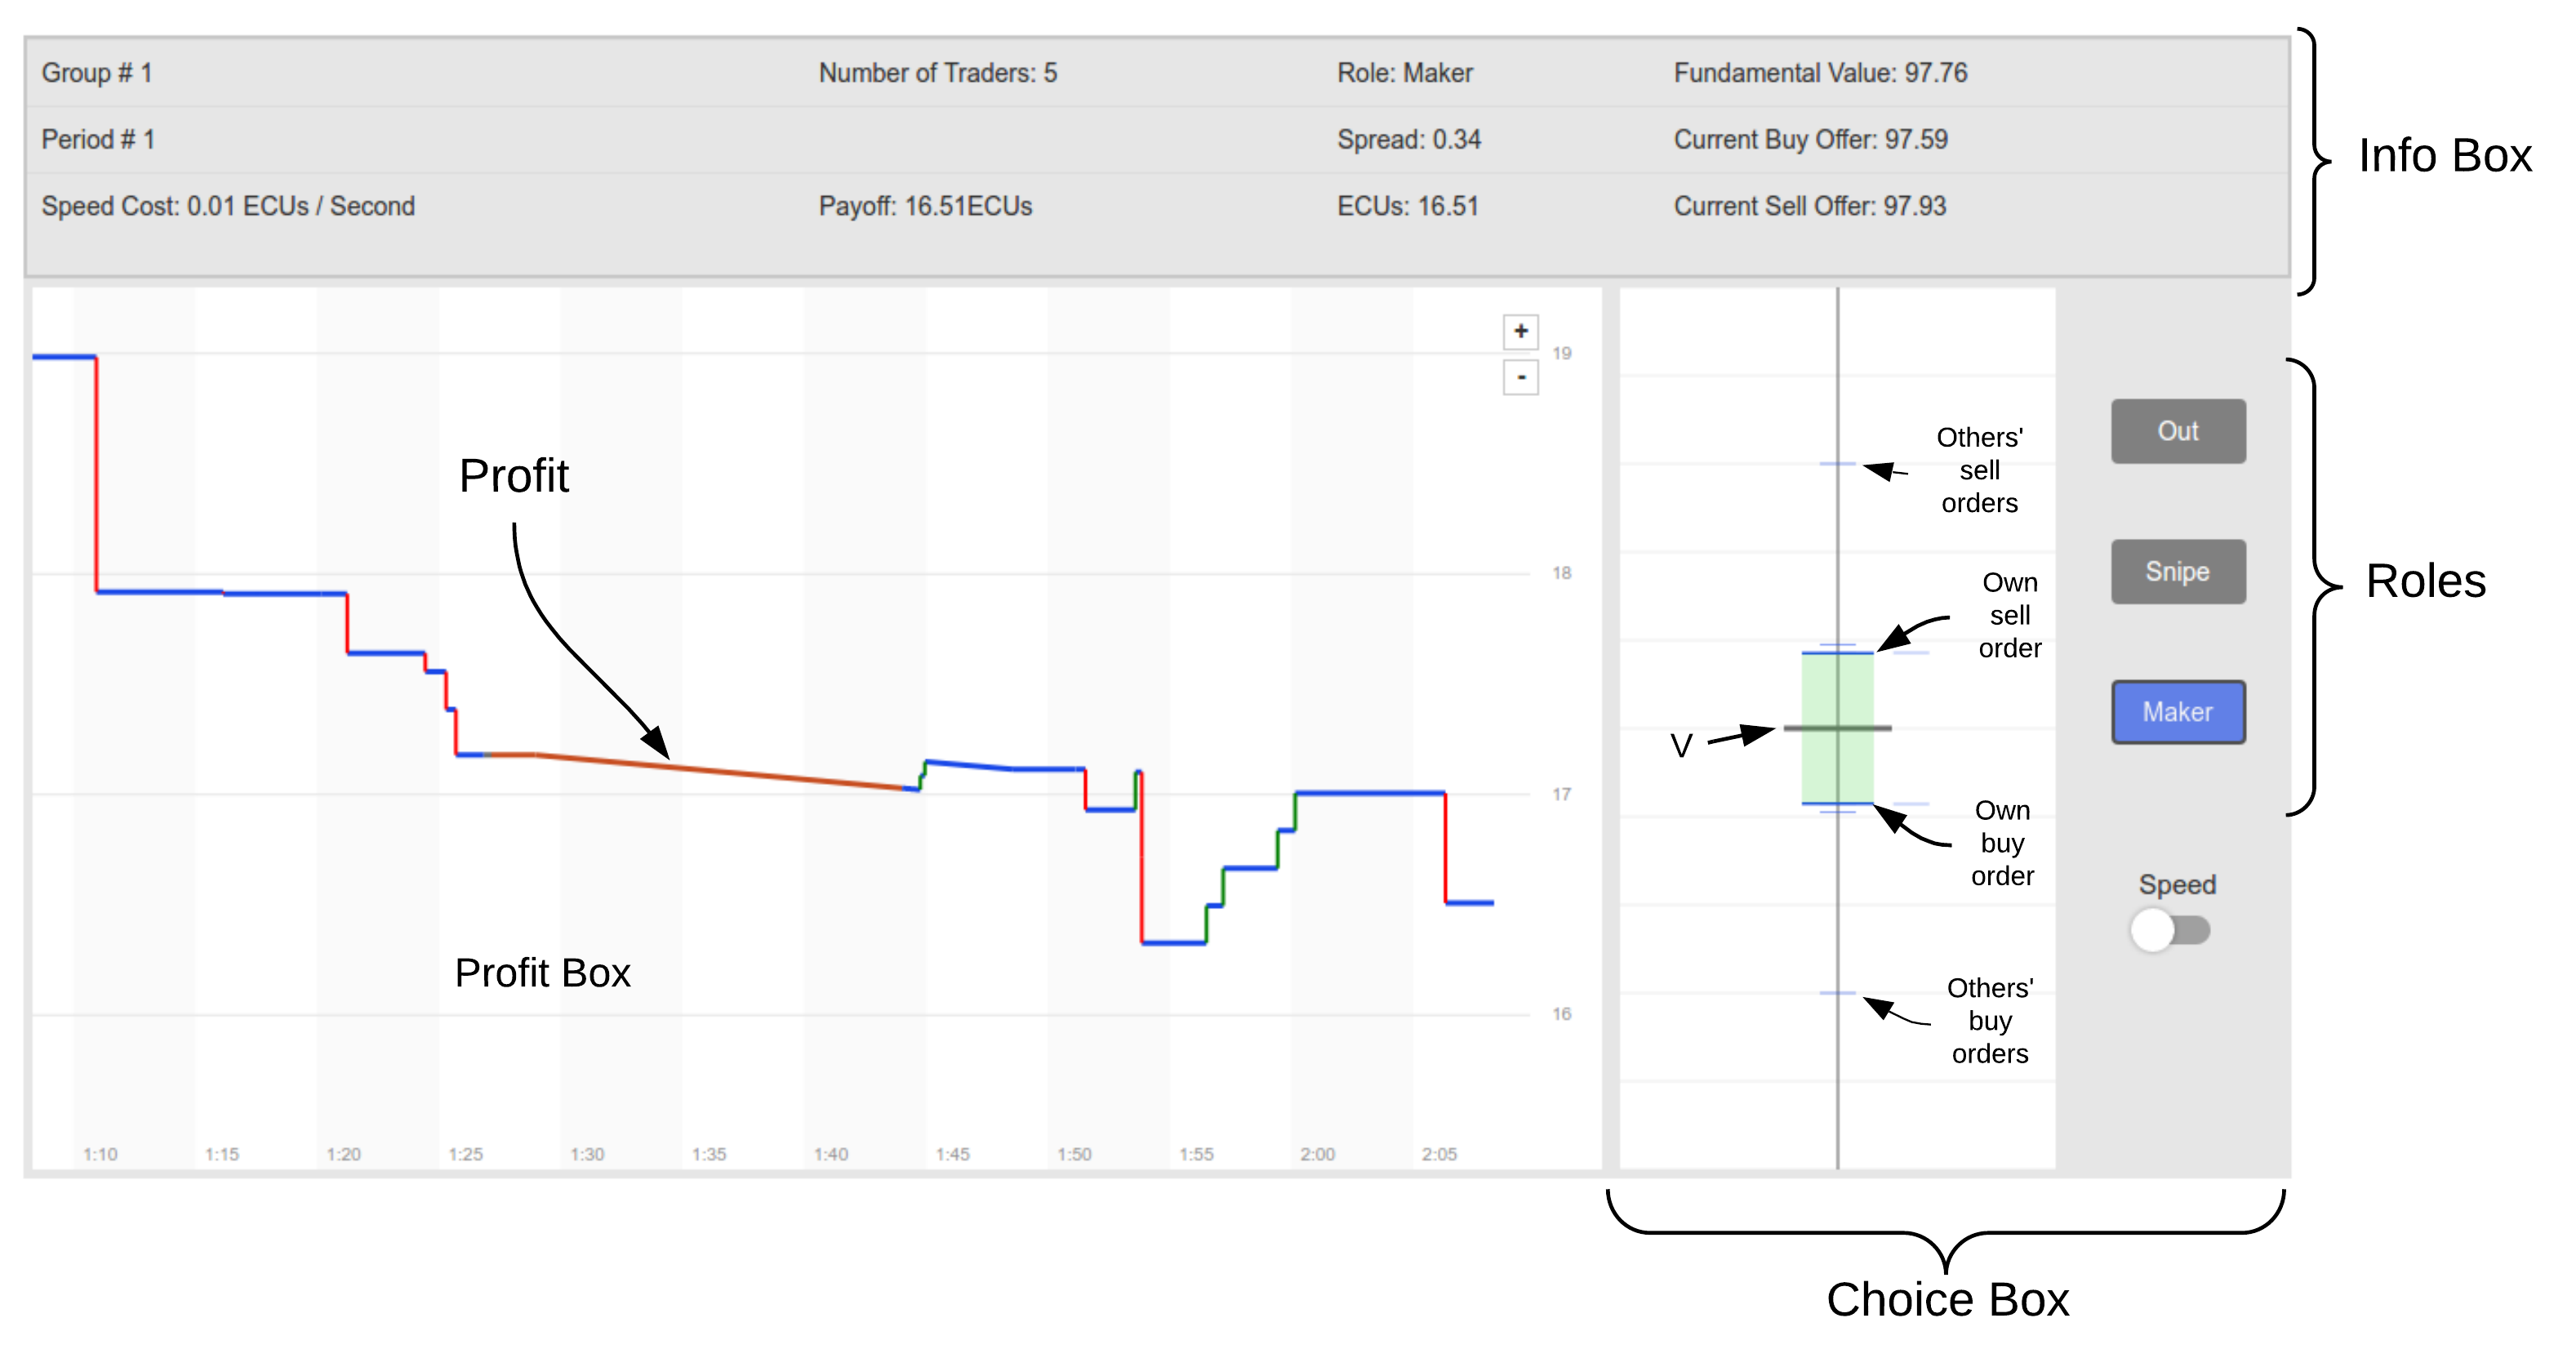
\includegraphics[width=1.06\textwidth]{img/UI-CDA_with_labels.png}
}

\frame{\frametitle{FBA User Interface}
%\begin{itemize}\item 
%\centering
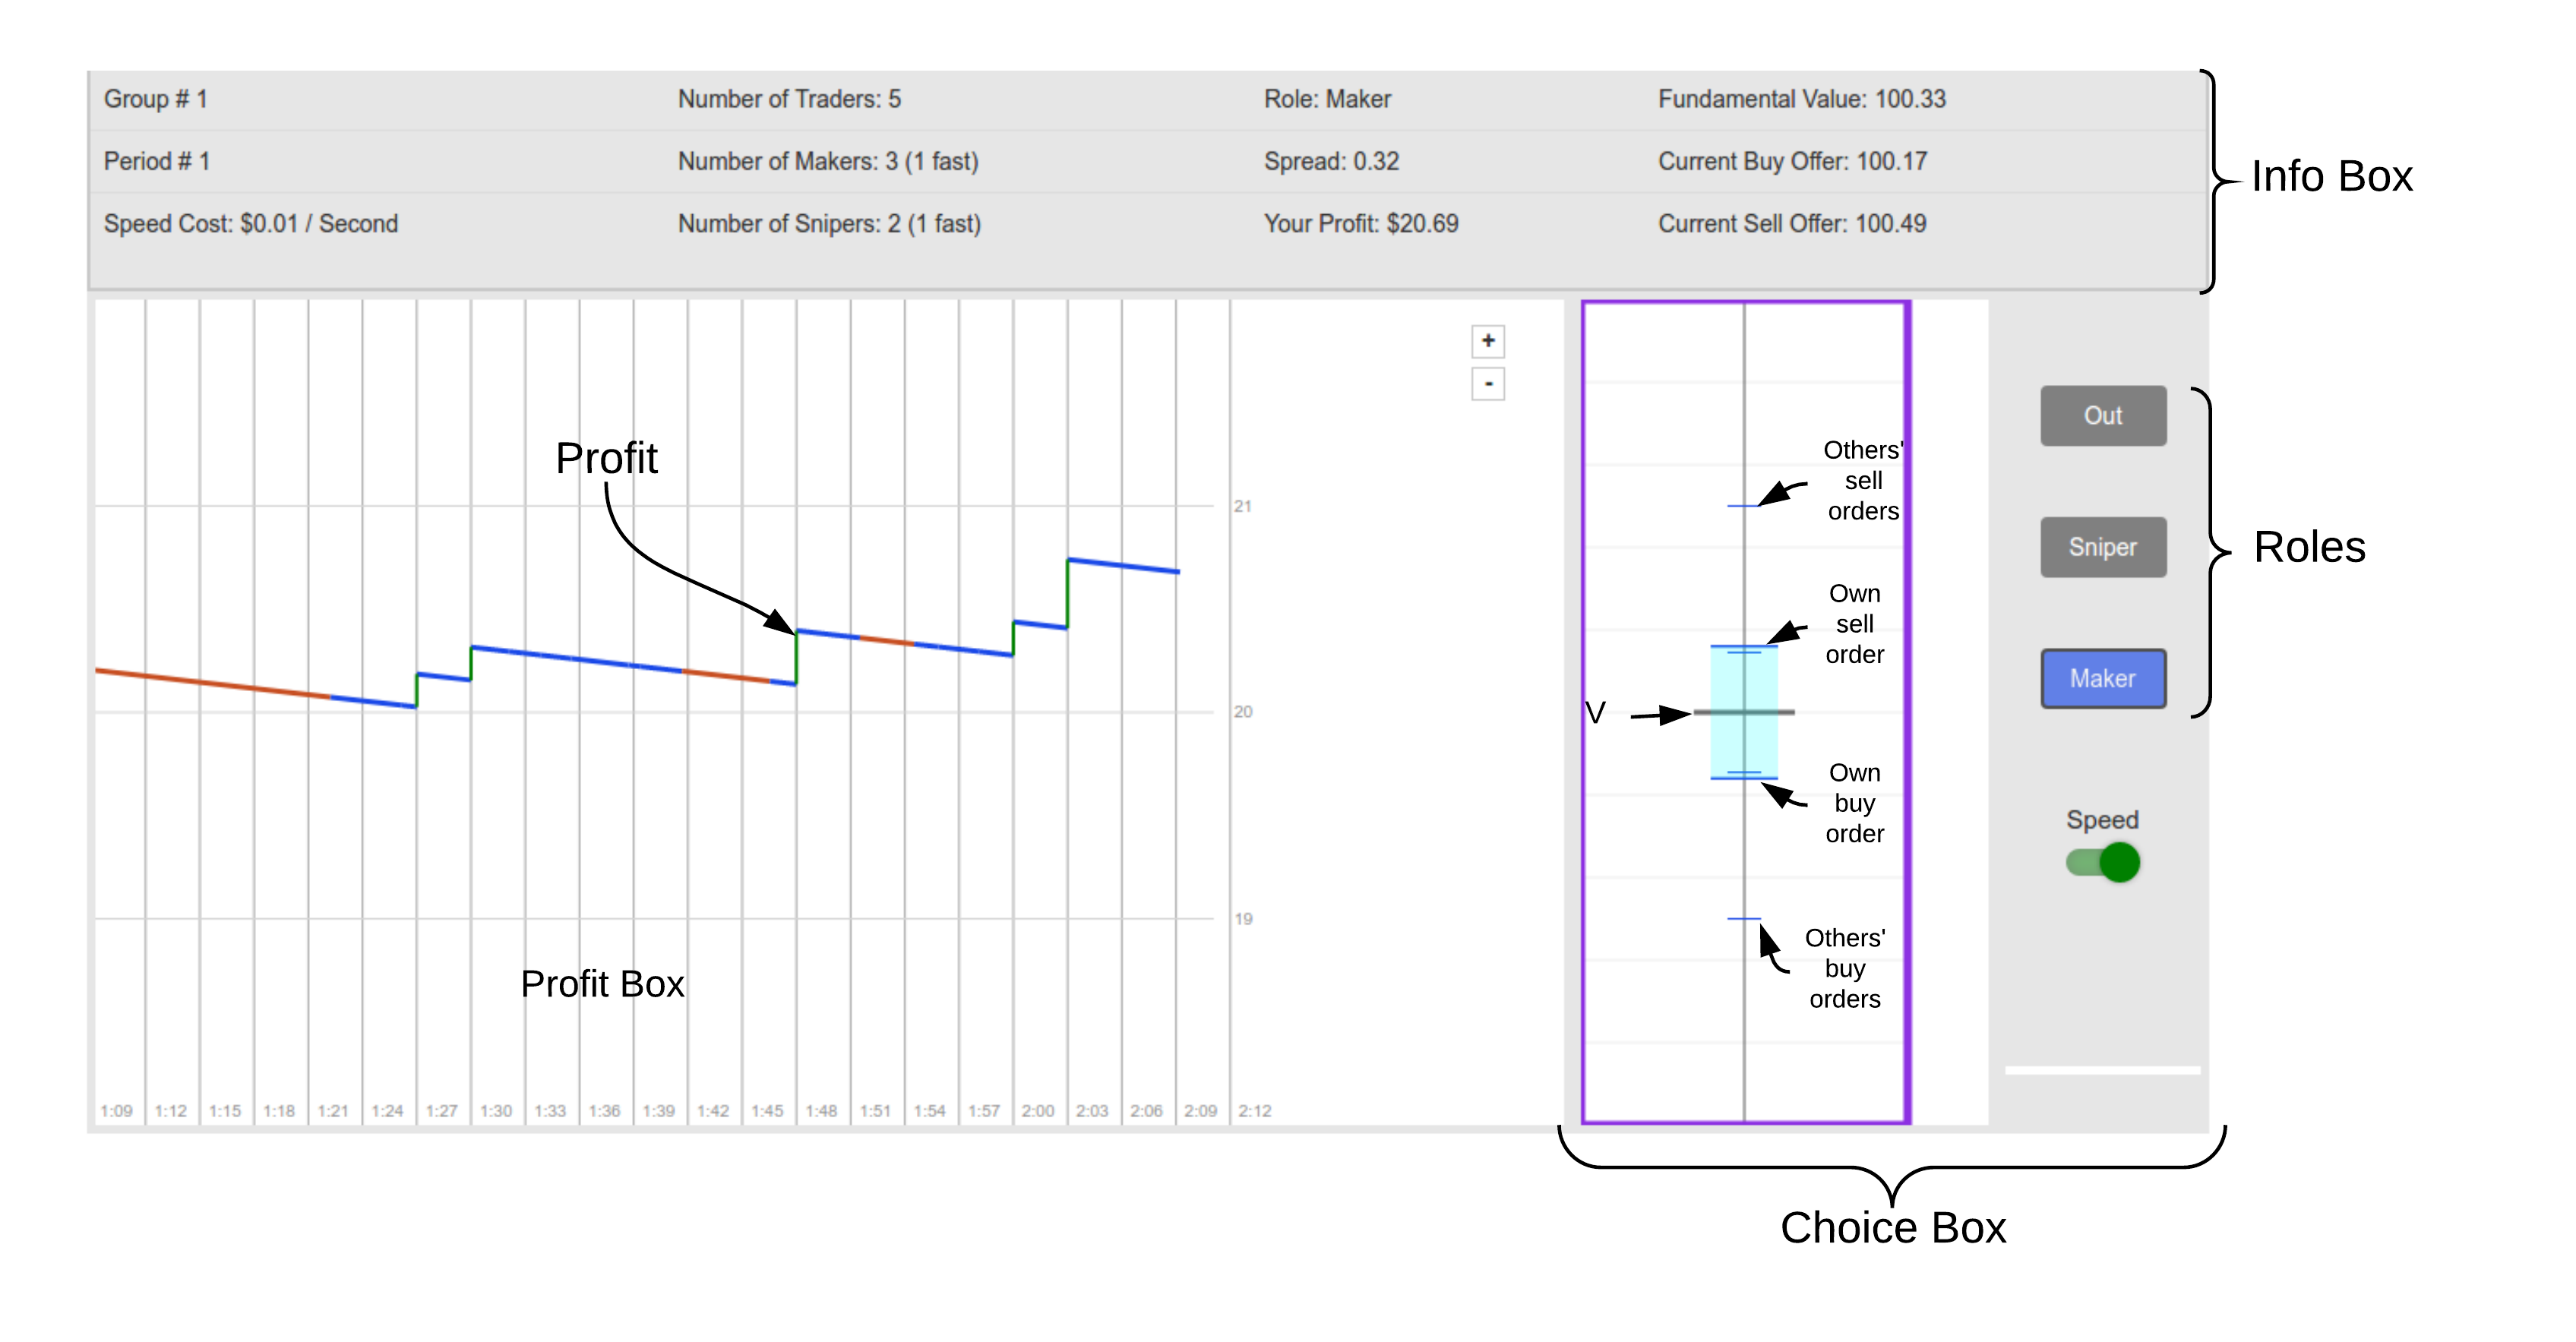
\includegraphics[width=1.06\textwidth]{img/UI-FBA.png}
}



\section{Results}

\subsection{Summary Stats}

%3.1 Subject choices
\frame{\frametitle{Results: Row Maker, Sniper, Speed, Spread} 
\begin{figure}
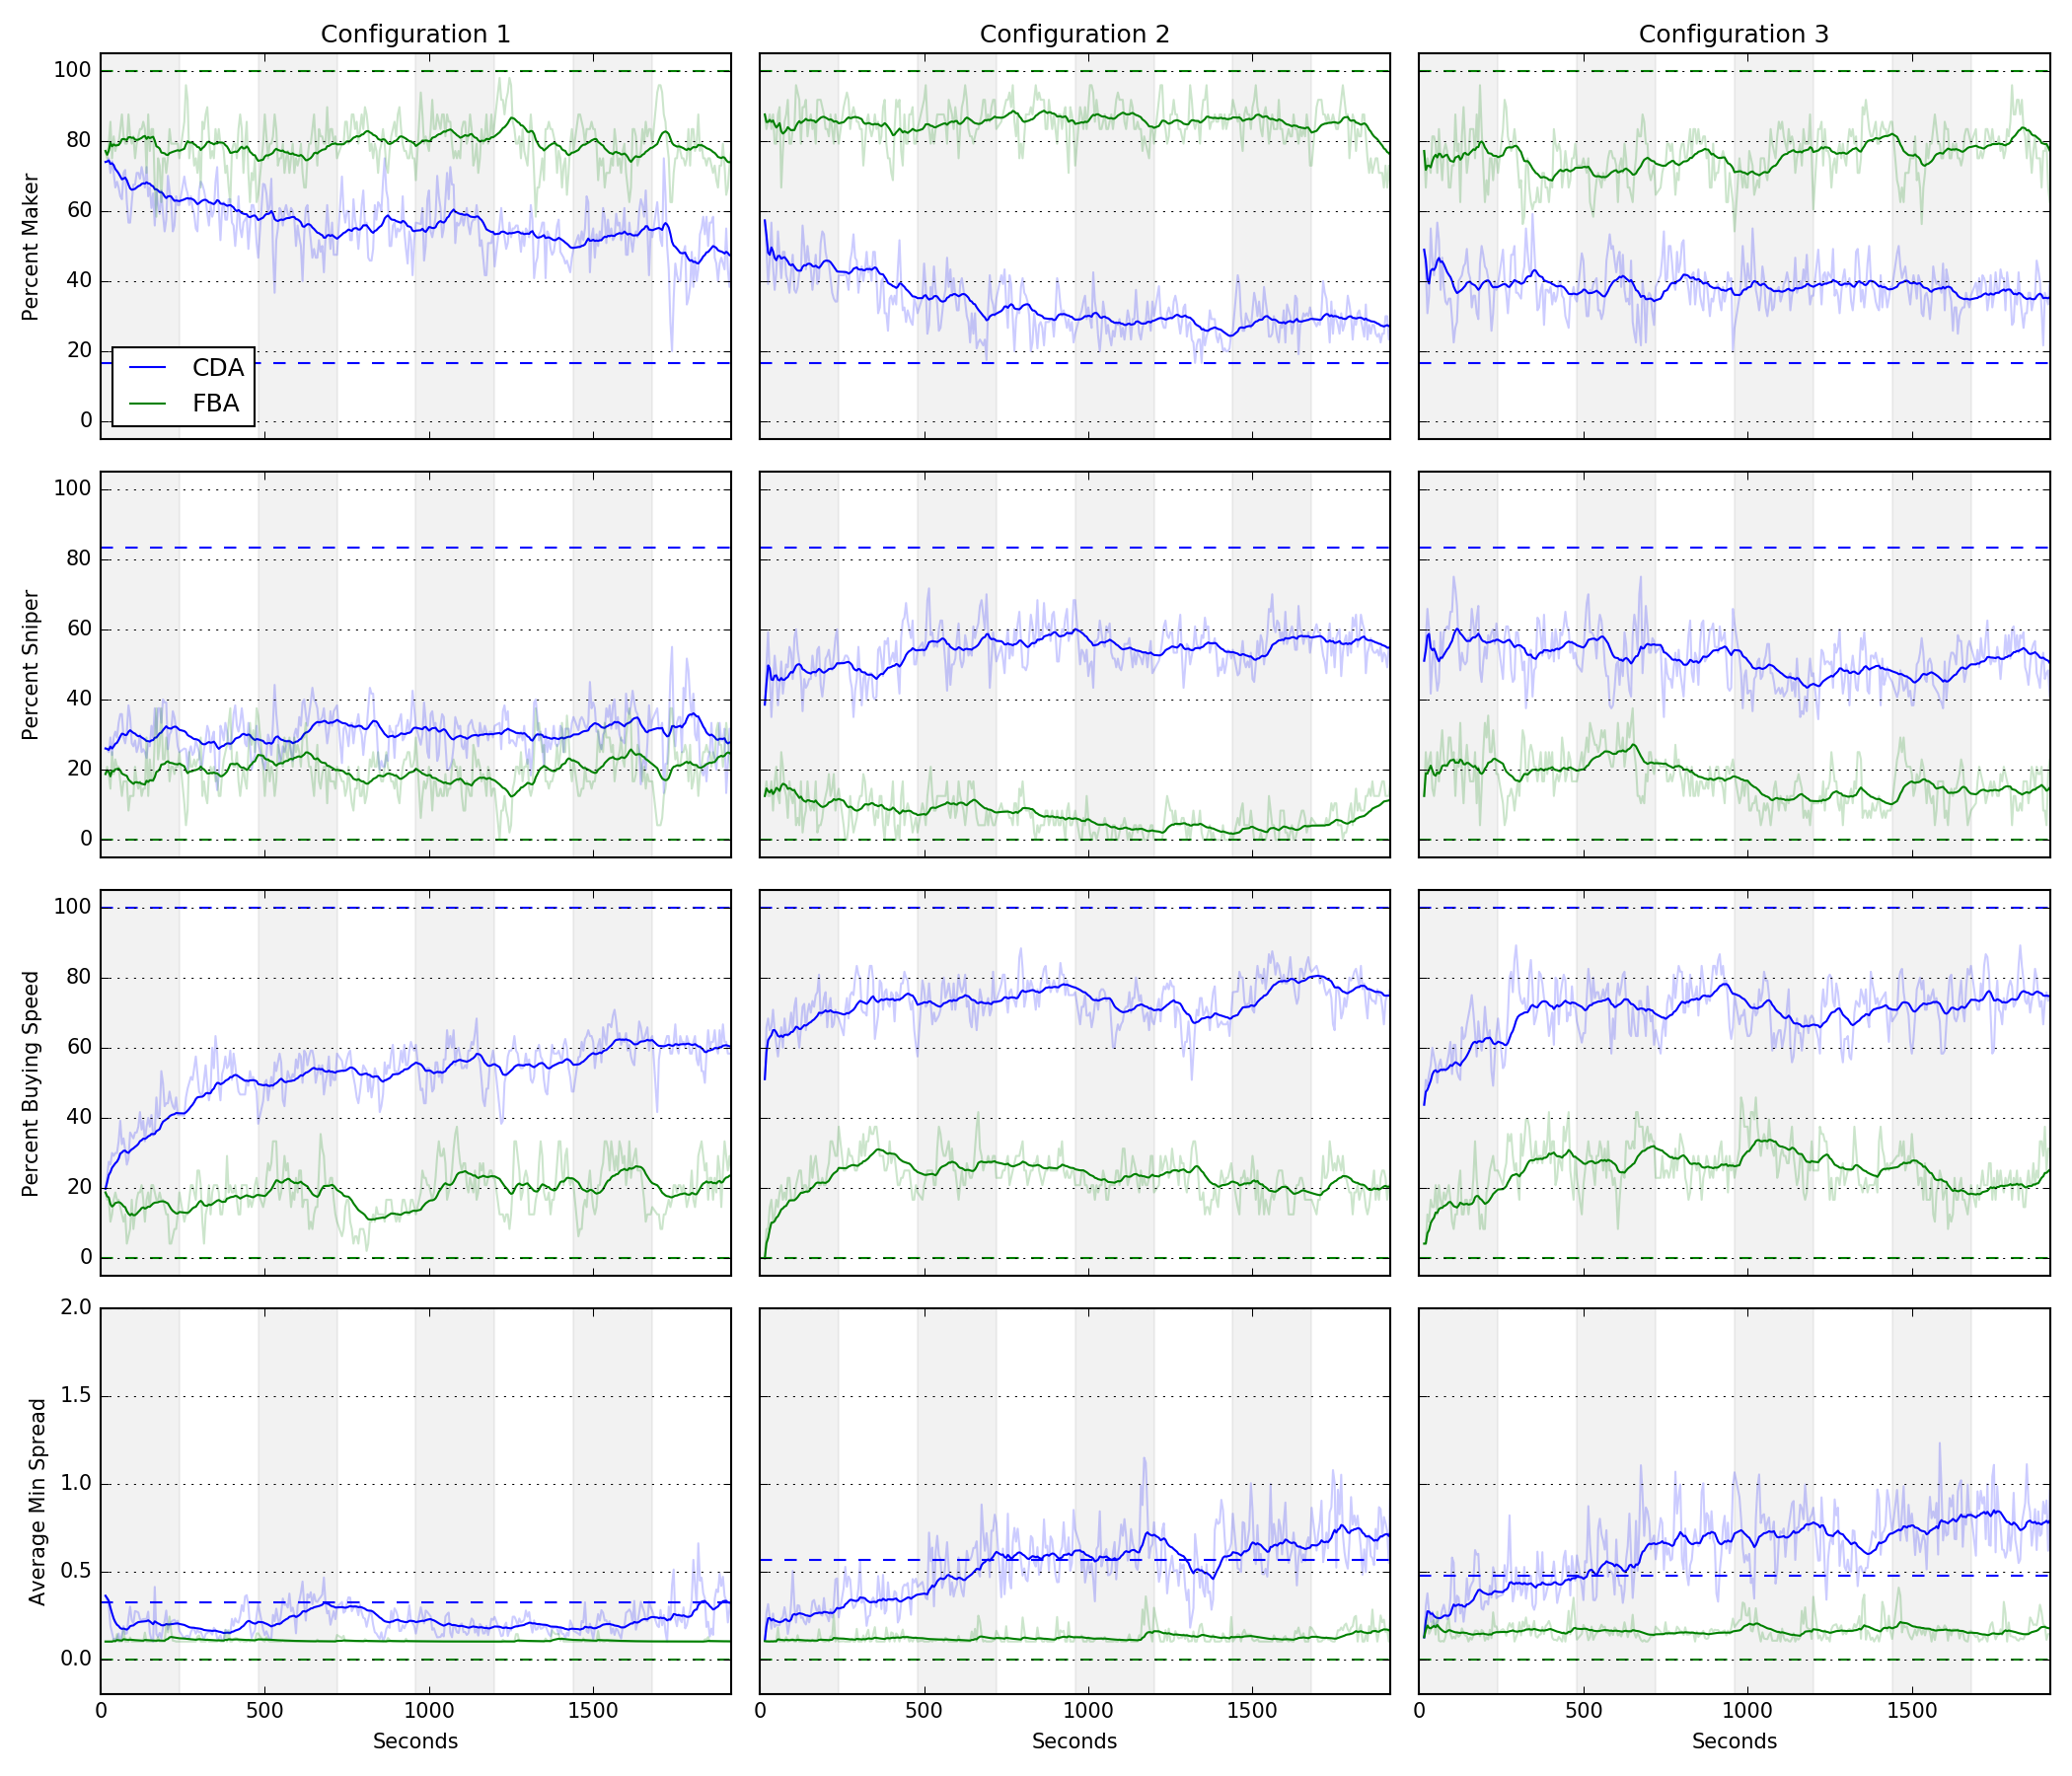
\includegraphics[width=0.70\textwidth]{img/allPlots.png}
\end{figure} 
}





\frame{\frametitle{Results: Summary statistics for choices} 
Choices
\begin{table}[]
\centering
%\caption{My caption}
\scalebox{.8}{
\begin{tabular}{llcccccc}
\hline
                     &             & Config 1 &        & Config 2 &        & Config 3 &        \\
                     &             & CDA      & FBA    & CDA      & FBA    & CDA      & FBA    \\ \hline
Making (\%)        &             &          &        &          &        &          &        \\
                     & Experiment  & 54    & 78.1  & 30.2    & 78.8  & 40.1    & 72.9 \\
                     & Equilibrium & 16.7    & 100 & 16.7    & 100 & 16.7    & 100 \\
Sniping (\%)         &             &          &        &          &        &          &        \\
                     & Experiment  & 31    & 20.8  & 58.1    & 14.5  & 49.5    & 14 \\
                     &  Equilibrium & 83.3    & 0   & 83.3    & 0  & 83.3    & 0   \\
Speed (\%)            &             &          &        &          &        &          &        \\
                     &  Experiment & 56.1    & 19.7  & 69    & 31.7  & 69.2    & 20.7 \\
                     & Equilibrium & 100   & 0  & 100   & 0   & 100  & 0   \\
Min. Spread &             &          &        &          &        &          &        \\
                    &  Experiment & 0.226    & 0.103  & 0.677    & 0.179  & 0.709    & 0.147  \\
                     & Equilibrium & 0.324    & 0 & 0.566    & 0  & 0.475    & 0  \\ \hline
\end{tabular}}
\end{table}
\begin{footnotesize}
% Panel (b) reports the average percentage of subjects acting as market makers, snipers, average percentage of subjects purchasing speed services, and the average minimum spread posted by market makers.
\end{footnotesize}
}

\frame{\frametitle{Results: Summary statistics for market} 
(c) Market Stats
\begin{table}[]
\centering
\scalebox{.7}{
\begin{tabular}{llcccccc}
\hline
                     &             & Config 1 &        & Config 2 &        & Config 3 &        \\
                     &             & CDA      & FBA    & CDA      & FBA    & CDA      & FBA    \\ \hline
$Std(P_t-P_{t-1})$        &             &          &        &          &        &          &        \\
                     &  Experiment & 2.51 & 0.561 & 4.62 & 1.00  & 6.68 & 1.11 \\
                     & Equilibrium & 0.241    & 0.289 & 0.276    & 0.327  & 0.235    & 0.430  \\
$Std(MinSpread)$         &             &          &        &          &        &          &        \\
                     &  Experiment & 0.204 & 0.0235 & 0.536 & 0.144 & 0.394 & 0.127 \\
                     & Equilibrium & 0    & 0 & 0    & 0  & 0    & 0  \\
Status Changes            &             &          &        &          &        &          &        \\
                    & Experiment & 20.5 & 6.26 & 31.6 & 6.26 & 17.0 & 7.34 \\
                     & Equilibrium & N/A   & 0 & N/A    & 0  & N/A    & 0  \\
$RMSD(P_t-V_t)$ &             &          &        &          &        &          &        \\
                    &  Experiment  & 0.347 & 0.212 & 0.512 & 0.410 & 0.460 & 0.381 \\
                     & Equilibrium & 0.223    & 0.136 & 0.329    & 0.211  & 0.372    & 0.276  \\ 
Transactions &             &          &        &          &        &          &        \\
                    & Experiment & 156 & 85.2 & 172 & 99.3 & 248 & 134 \\
  					 & Equilibrium & 106 & 80 & 100 & 48 & 147 & 120 \\
Period Profits &             &          &        &          &        &          &        \\
                    & Experiment  & .0869 & .435 & .603 & .372 & 4.31 &  1.52 \\
                     & Equilibrium & 0    & 0 & 0    & 0  & 0    & 0  \\ \hline
\end{tabular}}
\end{table}
}

\frame{\frametitle{Results: Summary} 

In choice data, the FBA exhibits:
\begin{itemize}
\item more traders choose to act as makers
\item fewer choose to act as snipers
\item fewer choose to purchase speed services
\item smaller market spreads 
\end{itemize}

In market level data, the FBA:
\begin{itemize}
\item reduces the volatility of transaction prices and spread
\item enhances price efficiency
\item results in more stable trader choices
\end{itemize}
}

\subsection{Regression Analysis}


\frame{\frametitle{Results: Regressions Analysis} 
To quantify treatment effects, we estimate the following model:
\begin{align}
y_{g,t}= \sum_{j=1}^{3}[\alpha_{j}Cj_{g,t}+\gamma_{j}Cj \times FBA_{g,t}] + \epsilon_{g,t},
\end{align}
where $y_{g,t} \hspace{0.1cm} \epsilon \hspace{0.1cm} \{Maker_{g,t}, Sniper_{g,t}, Speed_{g,t}, MinSpread_{g,t}\}$ is indexed by group and time, $Cj$ is a dummy variable for market configuration $j \hspace{0.1cm} \epsilon \hspace{0.1cm}$ \{1,2,3\} and $Cj \times FBA_{g,t}$ is the dummy variable indicating the interaction between configuration $j$ and the FBA format.
}

\frame{\frametitle{Results: Regressions Analysis} 
\begin{figure}
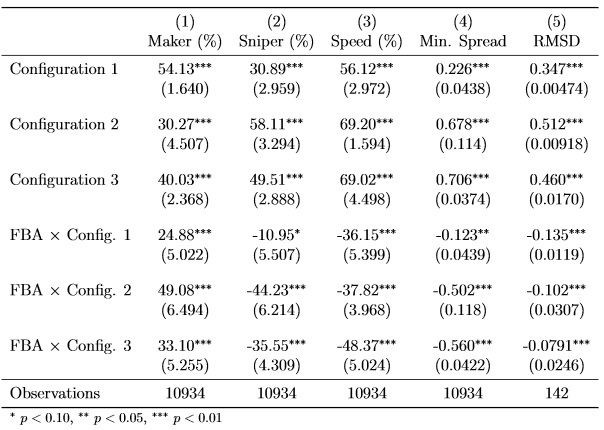
\includegraphics[width=0.7\textwidth]{img/Reg1_KL.jpg}
\end{figure} 
\begin{footnotesize}
\end{footnotesize}
}

\frame{\frametitle{Results: Regressions Analysis} 
Equilibrium behavior is rejected \\
However, the comparative statics of the differences between the two formats predicted by the model are confirmed in the data. \newline
Statistically, relative to the CDA:
\begin{itemize}
\item the FBA has more makers
\item the FBA has fewer snipers
\item the FBA has fewer traders purchasing speed technology
\item the FBA has lower minimum spreads
\item the FBA has lower RMSDs 
\end{itemize}
}


%%%%%%%%%%%%%%%%%%%%%%%%%%
\section{Conclusions and Next Steps}

\frame{\frametitle{Conclusions}
\begin{itemize}
\item Differences between FBA and CDA in the lab are consistent with comparative statics of the BCS model. 
\item FBA outperforms CDA in transaction costs (BCS environment). Effect sizes tend to be smaller than predicted.
\item Predatory behavior (sniping) is more prevalent in CDA than in FBA.
\item More turbulent markets in terms of stock value volatility (Config 2 and 3) exhibit difference between CDA and FBA formats more clearly  perhaps because more V-jump events.
\item Next Steps in the larger project (Cramton, Friedman, Ockenfels)
\end{itemize}
}


\frame{
\centering
{\huge Thank You} \\  
{\small \url{kristian@ucsc.edu} }

}


\frame{\frametitle{Transitory Market Dynamics}
To understand the dynamics of the market and the possible effects of transitory changes in the environment on subjects' decisions, we fit a vector autoregression of the form:
\begin{equation}
\mathbf{y}_{t}=\mathbf{a}+\mathbf{\Phi y}_{t-1}+\varepsilon_{t}
\end{equation}
\begin{equation}
\mathbf{y'}_{t}=[\%Sniper_{t}, \%Speed_{t}, MinSpread_{t}, Turbulence_{t}]
\end{equation}
}


\frame{\frametitle{Estimates of the constrained VAR(1)}
\begin{figure}
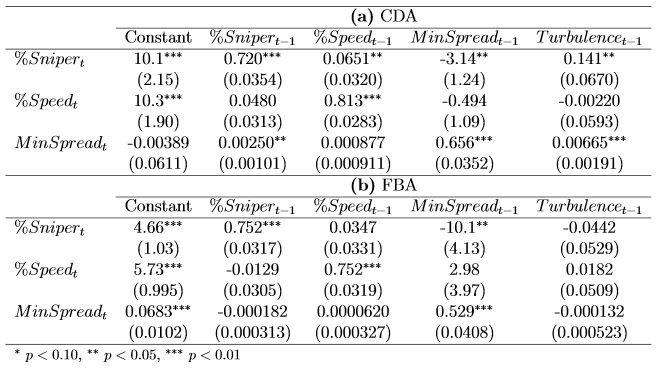
\includegraphics[width=0.75\textwidth]{img/Reg2_KL.jpg}
\begin{footnotesize}
\caption{Standard errors are reported in parentheses. Panel (a) reports CDA estimates and panel (b) 
reports FBA estimates.}
\end{footnotesize}
\end{figure} 
\begin{footnotesize}
The results show that very-short term, innovations in market conditions impact behavior in the CDA, while such effects of transient market changes do not exist in the FBA.
\end{footnotesize}
}


\frame{\frametitle{Transitory Market Dynamics}
\begin{figure}
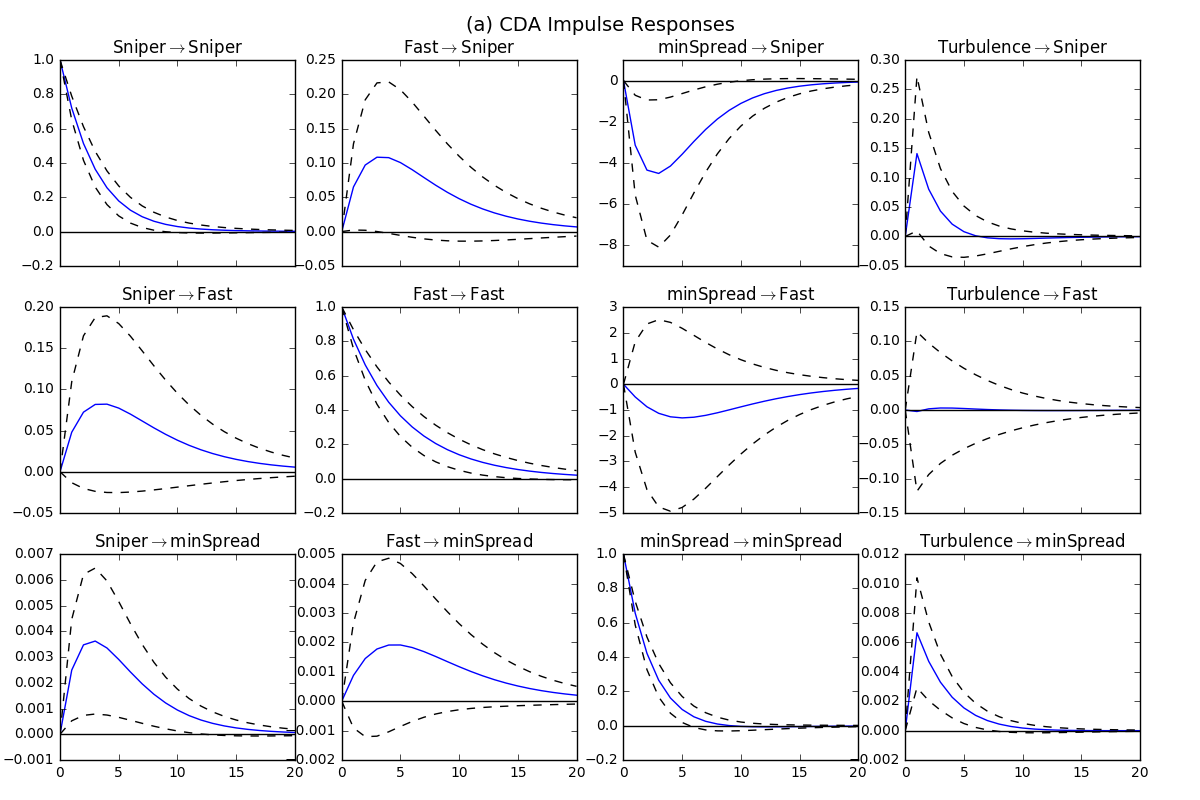
\includegraphics[width=0.80\textwidth]{img/irfCDA.png}
\caption{Unit impulse responses for the estimated VAR under CDA.}
\end{figure} 
}

\frame{\frametitle{Transitory Market Dynamics}
\begin{figure}
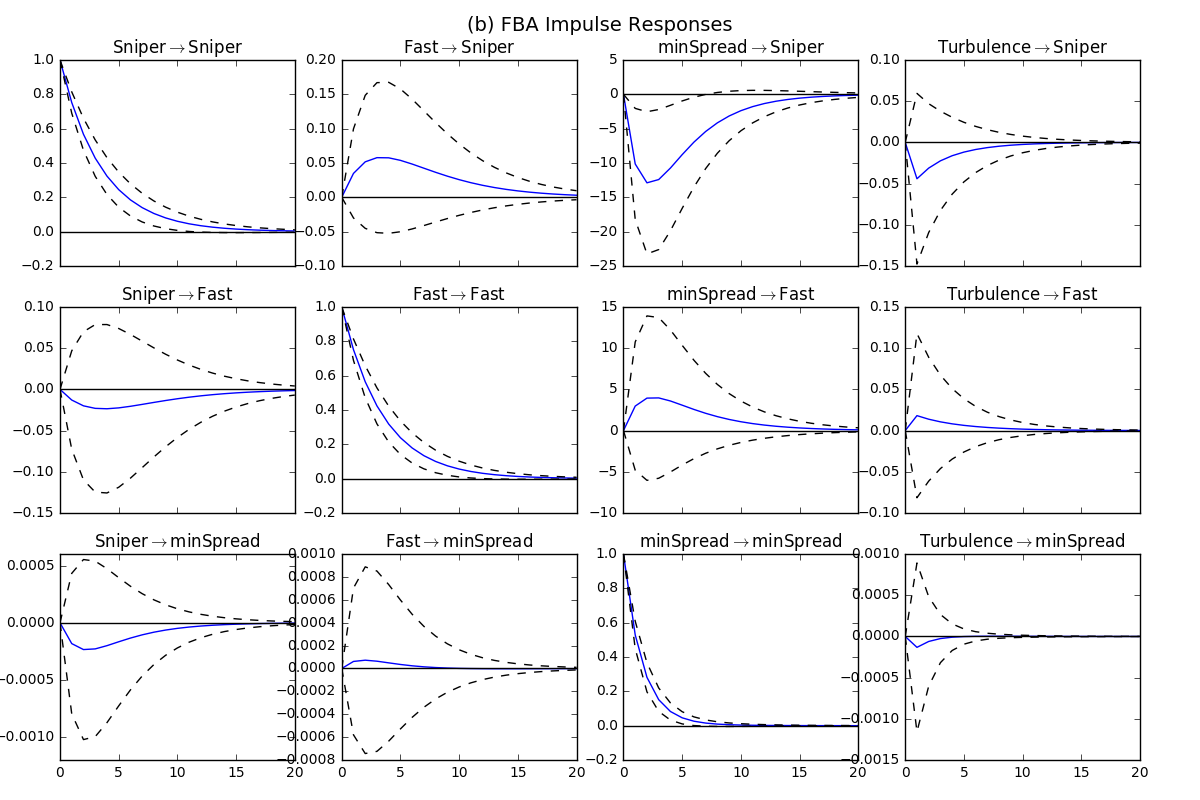
\includegraphics[width=0.80\textwidth]{img/irfFBA.png}
\caption{Unit impulse responses for the estimated VAR under FBA.}
\end{figure} 
}




\end{document}



